\documentclass[10pt,a4paper]{article}

\usepackage[italian]{babel}
\usepackage[usenames,dvipsnames,table]{xcolor}
\usepackage[utf8]{inputenc}
\usepackage[T1]{fontenc}
\usepackage{soul}
\usepackage[a4paper, portrait, margin=2.5cm]{geometry}
\usepackage{array}
\usepackage{tabularx} 
\usepackage{booktabs}
\usepackage{multicol}
\usepackage{amsmath}
\usepackage{amsfonts}
\usepackage{amssymb}
\usepackage{algorithmicx}
\usepackage[noend]{algpseudocode}
\usepackage{wrapfig}
\usepackage{graphicx}
\usepackage{hyperref}
\usepackage{listings}
\usepackage{mdframed}

\lstset{basicstyle=\ttfamily}

\graphicspath{ {./images/} }

\begin{document}

\title{Data Flow Analysis \\
\large Assignment 2}
\author{Iacopo Ruzzier, Daniele Fassetta, Anna Semeraro}

\maketitle
\tableofcontents

\newpage

\section{Very Busy Expressions}
\subsection{Definizione del problema}

\begin{itemize}
  \item Un'espressione \`e \textbf{very busy} in un punto \textit{p} se, indipendentemente dal percorso preso da \textit{p}, l'espressione viene usata prima che uno dei suoi operandi venga definito.
  \item Un'espressione \lstinline|a+b| \`e \textbf{very busy} in un punto \textit{p} se \lstinline|a+b| \`e valutata in tutti i percorsi da \textit{p} a \textit{Exit} e non c'\`e una definizione di \lstinline|a| o \lstinline|b| lungo tali percorsi
\end{itemize}


\begin{table}[h!]
  \centering
  \begin{tabular}{|l|p{4cm}|}
    \hline
    \textbf{} & \textbf{Very Busy Expressions} \\
    \hline
    Domain & Expressions\\
    \hline
    Direction & Backward\newline $in[b]=f_{b}(out[b])$\newline $out[b]=\wedge\, in(succ[b])$\\
    \hline
    Transfer function & $f_b = Gen_b \cup (x - Kill_b) $\\
    \hline
    Meet Operation ($\land$) & $\cap$ \\
    \hline
    Boundary Condition & $in[exit] = \emptyset$ \\
    \hline
    Initial interior points & $in[b] = \mathcal{U}$ \\
    \hline
  \end{tabular}
  \caption{Very busy expressions}
\end{table}

Dove
\begin{itemize}
  \item $Gen[b]$: espressioni valutate all'interno del Basic Block
  \item $Kill[b]$: un'espressione viene uccisa quando un suo operando viene ridefinito all'interno di \textit{b}
\end{itemize}

\subsection{Esempio di esecuzione}

\begin{minipage}[c]{.25\textwidth}
  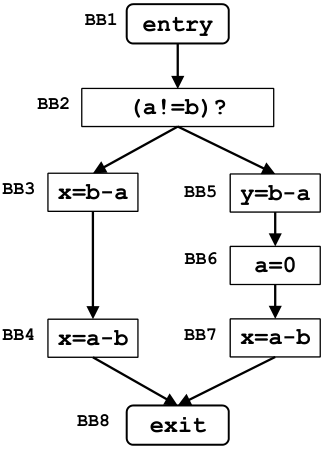
\includegraphics[width=\textwidth]{example-1.png}
\end{minipage}
\begin{minipage}[c]{.5\textwidth}
\renewcommand{\arraystretch}{1.5}
\rowcolors{2}{gray!10}{white}
\begin{tabular}{|c|l|l|}
\hline
\rowcolor{blue!30}
BB & \multicolumn{2}{c|}{Iterazione 1} \\
\hline
\rowcolor{blue!30}
   & $OUT[B] = \wedge\, IN(succ[b])$ & $IN[B] = Gen[B] \cup (OUT[B] - Kill[B])$ \\
\hline
BB7 & $\emptyset$ (\textbf{boundary condition}) & $a-b \cup (\emptyset - \emptyset) = a-b$ \\
\hline
BB6 & $a-b$ & $\emptyset \cup (\lbrace a-b\rbrace - \lbrace a-b, b-a\rbrace)=\emptyset$ \\
\hline
BB5 & $\emptyset$ & $b-a \cup (\emptyset - \emptyset) = b-a$ \\
\hline
BB4 & $\emptyset$ & $a-b \cup (\emptyset - \emptyset) = a-b$ \\
\hline
BB3 & $a-b$ & $b-a \cup (\lbrace a-b\rbrace - \emptyset) =\lbrace b-a,a-b\rbrace$ \\
\hline
BB2 & $\lbrace b-a\rbrace\cap \lbrace a-a,a-b\rbrace = b-a$ & $\emptyset \cup (\lbrace b-a\rbrace - \emptyset) = b-a$ \\
\hline
BB1 & $\boxed{b-a}$ & / \\
\hline
\end{tabular}
\end{minipage}

\newpage
\section{Dominator Analysis}
\subsection{Definizione del problema}

\begin{itemize}
  \item In un CFG diciamo che un nodo \textit{X} \textbf{domina} un altro nodo \textit{Y} se il nodo \textit{X} appare in ogni percorso del grafo che porta dal blocco \textit{Entry} al blocco \textit{Y}
  \item annotiamo ogni basic block $B_{i}$ con un insieme $Dom[B_{i}]$:
  \begin{itemize}
    \item $B_{i}\in Dom[B_{j}] \iff B_{i}$ domina $B_{j}$
    \item $B_{i}\in Dom[B_{i}]$: per definizione un nodo domina se stesso
  \end{itemize}
  
\end{itemize}


\begin{table}[h!]
  \centering
  \begin{tabular}{|l|p{4cm}|}
    \hline
    \textbf{} & \textbf{Dominator Analysis} \\
    \hline
    Domain & Basic Blocks\\
    \hline
    Direction & Forward\newline $out[b]=f_{b}(in[b])$\newline $in[b]=\wedge\, out(pred[b])$\\
    \hline
    Transfer function & $f_b = Dom[b] = b \cup x$\\
    \hline
    Meet Operation (\(\land\)) & $\cap$ \\
    \hline
    Boundary Condition & $out[entry] = entry $\\
    \hline
    Initial interior points & $out[b] = \mathcal{U} $ \\
    \hline
  \end{tabular}
  \caption{Dominator analysis}
\end{table}

\subsection{Esempio di esecuzione}

\noindent\begin{minipage}[c]{.4\textwidth}
  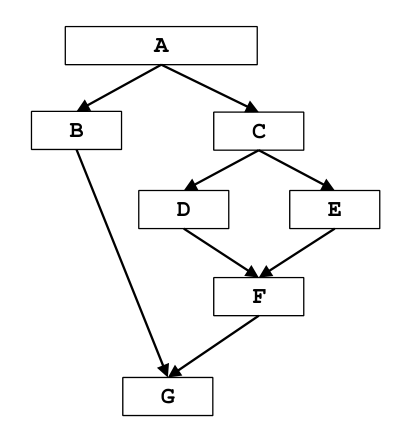
\includegraphics[width=.7\textwidth]{example-2.png}
\end{minipage}
\begin{minipage}[c]{.5\textwidth}
\centering
\renewcommand{\arraystretch}{1.5}
\rowcolors{2}{gray!10}{white}
\begin{tabular}{|c|l|l|}
\hline
\rowcolor{blue!30}
BB & \multicolumn{2}{c|}{Iterazione 1} \\
\hline
\rowcolor{blue!30}
   & $IN[B] = \wedge\, OUT(pred[b])$ & $DOM[B]= B \cup IN[B]$ \\
\hline
A & $\emptyset$ (\textbf{boundary condition}) & $A \cup \emptyset = A$ \\
\hline
B & $A$ & $B \cup A=\lbrace A,B \rbrace$ \\
\hline
C & $A$ & $C \cup A = \lbrace A,C \rbrace$ \\
\hline
D & $\lbrace A,C \rbrace$ & $D \cup \lbrace A,C \rbrace = \lbrace A,C,D \rbrace$ \\
\hline
E & $\lbrace A,C \rbrace$ & $E \cup \lbrace A,C \rbrace = \lbrace A,C,E \rbrace$ \\
\hline
F & $\lbrace A,C,D\rbrace\cap \lbrace A,C,E\rbrace = \lbrace A,C \rbrace$ & $F \cup \lbrace A,C\rbrace = \lbrace A,C,F\rbrace$ \\
\hline
G & $\lbrace A,B \rbrace \cap \lbrace A,C,F\rbrace = A$ & $G \cup A = \lbrace A,G \rbrace$ \\
\hline
\end{tabular}
\end{minipage}

\newpage
\section{Constant propagation}

\subsection{Definizione del problema}

\begin{itemize}
  \item L'obiettivo della \textit{constant propagation} \`e quello di determinare in quali punti del programma le variabili hanno un valore costante.
  \item L'informazione da calcolare per ogni nodo del CFG \`e un insieme di coppie del tipo\\\lstinline|<variabile,valore costante>|.
  \item Se abbiamo la coppia \lstinline|<x,c>| al nodo \textit{n}, significa che \lstinline|x| \`e garantito avere il valore \lstinline|c| ogni volta che \textit{n} viene raggiunto durante l'esecuzione del programma.
\end{itemize}


\begin{table}[h!]
  \centering
  \begin{tabular}{|l|p{4cm}|}
    \hline
    \textbf{} & \textbf{Constant Propagation} \\
    \hline
    Domain & pairs $(v,c)$\\
    \hline
    Direction & Forward\newline $out[b]=f_{b}(in[b])$ \newline $in[b] = \wedge\, out(pred[b])$ \\
    \hline
    Transfer function & $f_{b}=Gen[b] \cup (x - Kill[b])$ \\
    \hline
    Meet Operation (\(\land\)) & $\cap$\\
    \hline
    Boundary Condition & $out[entry]=\emptyset$ \\
    \hline
    Initial interior points & $out[b]=\mathcal{U}$ \\
    \hline
  \end{tabular}
  \caption{Constant propagation}
\end{table}

\begin{itemize}
  \item $Gen[b]$ rappresenta l'insieme di nuovi assegnamenti (all'interno di \textit{b}) con valore costante. I casi di interesse sono:
\begin{itemize}
  \item \lstinline|x = c| con \lstinline|c| costante: $Gen[b] = Gen[b] \cup (x,c)$
  \item \lstinline|x = c1|$\oplus$\lstinline|c2| con \lstinline|c1,c2| costanti: $Gen[b] = Gen[b] \cup (x,c1\oplus c2)$ (calcolando il valore dell'espressione)
  \item \lstinline|x = c|$\oplus$\lstinline|y| o \lstinline|x = y|$\oplus$\lstinline|c| con \lstinline|c| costante:
\begin{enumerate}
  \item controlliamo che y sia presente nell'insieme in input: $\exists (y,v_{y}) \in In[b]$
  \item se \`e vero, $Gen[b] = Gen[b] \cup (x,e)$ con $e = c\oplus v_{y}$ (o $v_{y}\oplus c$)
\end{enumerate}
\item \lstinline|x = y|$\oplus$\lstinline|z|, valutando \lstinline|y| e \lstinline|z| allo stesso modo del caso precedente:
  \begin{equation*}
    \exists (y,v_{y}), (z,v_{z})\in In[b] \implies Gen[b] = Gen[b] \cup (x,e) \text{~con~} e=v_{y}\oplus v_{z}
  \end{equation*}

\begin{mdframed}
  Nel caso di definizioni multiple di \lstinline|x|, riteniamo valida solamente l'ultima all'interno di \textit{b}
\end{mdframed}
\end{itemize}
\item $Kill[b]$: ogni definizione \lstinline|x = expr| uccide le coppie $(x,c)\in \mathcal{D}$ (dominio)
\end{itemize}

\subsection{Esempio di esecuzione}

\begin{figure}[h!]
  \centering
  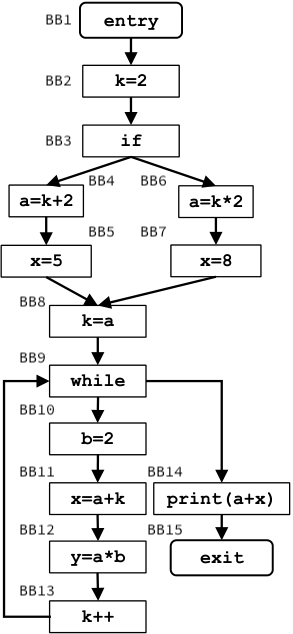
\includegraphics[width=.3\textwidth]{example-3.png}
\end{figure}

\begin{table}[h!]
\centering
\renewcommand{\arraystretch}{1.2}
\rowcolors{2}{gray!10}{white}
\begin{tabular}{|c|c|c|}
\hline
\rowcolor{blue!30}
 & \multicolumn{2}{c|}{Iterazione 1} \\
 \hline
\rowcolor{blue!30}
 & IN[B] & OUT[B] \\
\hline
BB1 & $\emptyset$ & $\emptyset$ \\
\hline
BB2 & $\emptyset$ & $\lbrace(k,2)\rbrace$ \\
\hline
BB3 & $\lbrace(k,2)\rbrace$ & $\lbrace(k,2)\rbrace$ \\
\hline
BB4 & $\lbrace(k,2)\rbrace$ & $\lbrace(k,2),(a,4)\rbrace$ \\
\hline
BB5 & $\lbrace(k,2),(a,4)\rbrace$ & $\lbrace(k,2),(a,4),(x,5)\rbrace$ \\
\hline
BB6 & $\lbrace(k,2)\rbrace$ & $\lbrace(k,2),(a,4)\rbrace$ \\
\hline
BB7 & $\lbrace(k,2),(a,4)\rbrace$ & $\lbrace(k,2),(a,4),(x,8)\rbrace$ \\
\hline
BB8 & $\lbrace(k,2),(a,4)\rbrace$ & $\lbrace(k,4),(a,4)\rbrace$ \\
\hline
BB9 & $\lbrace(k,4),(a,4)\rbrace\cap\mathcal{U}=\lbrace(k,4),(a,4)\rbrace$ & $\lbrace(k,4),(a,4)\rbrace$ \\
\hline
BB10 & $\lbrace(k,4),(a,4)\rbrace$ & $\lbrace(k,4),(a,4),(b,2)\rbrace$\\
\hline
BB11 & $\lbrace(k,4),(a,4),(b,2)\rbrace$ & $\lbrace(k,4),(a,4),(b,2),(x,8)\rbrace$ \\
\hline
BB12 & $\lbrace(k,4),(a,4),(b,2),(x,8)\rbrace$ & $\lbrace(k,4),(a,4),(b,2),(x,8),(y,8)\rbrace$ \\
\hline
BB13 & $\lbrace(k,4),(a,4),(b,2),(x,8),(y,8)\rbrace$ & $\lbrace(k,5),(a,4),(b,2),(x,8),(y,8)\rbrace$ \\
\hline
BB14 & $\lbrace(k,4),(a,4)\rbrace$ & $\lbrace(k,4),(a,4)\rbrace$ \\
\hline
BB15 & $\lbrace(k,4),(a,4)\rbrace$ & $\lbrace(k,4),(a,4)\rbrace$ \\
\hline
\end{tabular}
\end{table}

\begin{table}[h!]
\centering
\renewcommand{\arraystretch}{1.2}
\rowcolors{2}{gray!10}{white}
\begin{tabular}{|c|c|c|}
\hline
\rowcolor{blue!30}
  & \multicolumn{2}{c|}{Iterazione 2} \\
  \hline
\rowcolor{blue!30}
  & IN[B] & OUT[B] \\
\hline
BB1 & $\emptyset$ & $\emptyset$ \\
\hline
BB2 & $\emptyset$ & $\lbrace(k,2)\rbrace$ \\
\hline
BB3 & $\lbrace(k,2)\rbrace$ & $\lbrace(k,2)\rbrace$ \\
\hline
BB4 & $\lbrace(k,2)\rbrace$ & $\lbrace(k,2),(a,4)\rbrace$ \\
\hline
BB5 & $\lbrace(k,2),(a,4)\rbrace$ & $\lbrace(k,2),(a,4),(x,5)\rbrace$ \\
\hline
BB6 & $\lbrace(k,2)\rbrace$ & $\lbrace(k,2),(a,4)\rbrace$ \\
\hline
BB7 & $\lbrace(k,2),(a,4)\rbrace$ & $\lbrace(k,2),(a,4),(x,8)\rbrace$ \\
\hline
BB8 & $\lbrace(k,2),(a,4)\rbrace$ & $\lbrace(k,4),(a,4)\rbrace$ \\
\hline
BB9 & $\lbrace(k,4),(a,4)\rbrace\cap\lbrace(y,8),(k,5),(a,4),(b,2)(x,8)\rbrace=\lbrace(a,4)\rbrace$ & $\lbrace(a,4)\rbrace$ \\
\hline
BB10 & $\lbrace(a,4)\rbrace$ & $\lbrace(a,4),(b,2)\rbrace$\\
\hline
BB11 & $\lbrace(a,4),(b,2)\rbrace$ & $\lbrace(a,4),(b,2)\rbrace$ \\
\hline
BB12 & $\lbrace(a,4),(b,2)\rbrace$ & $\lbrace(a,4),(b,2),(y,8)\rbrace$ \\
\hline
BB13 & $\lbrace(a,4),(b,2),(y,8)\rbrace$ & $\lbrace(a,4),(b,2),(y,8)\rbrace$ \\
\hline
BB14 & $\lbrace(a,4),(b,2),(y,8)\rbrace$ & $\lbrace(a,4),(b,2),(y,8)\rbrace$ \\
\hline
BB15 & $\lbrace(a,4),(b,2),(y,8)\rbrace$ & $\lbrace(a,4),(b,2),(y,8)\rbrace$ \\
\hline
\end{tabular}
\end{table}

\begin{table}[h!]
  \centering
  \renewcommand{\arraystretch}{1.2}
  \rowcolors{2}{gray!10}{white}
  \begin{tabular}{|c|c|c|}
  \hline
  \rowcolor{blue!30}
    & \multicolumn{2}{c|}{Iterazione 3} \\
    \hline
  \rowcolor{blue!30}
    & IN[B] & OUT[B] \\
  \hline
  BB1 & $\emptyset$ & $\emptyset$ \\
  \hline
  BB2 & $\emptyset$ & $\lbrace(k,2)\rbrace$ \\
  \hline
  BB3 & $\lbrace(k,2)\rbrace$ & $\lbrace(k,2)\rbrace$ \\
  \hline
  BB4 & $\lbrace(k,2)\rbrace$ & $\lbrace(k,2),(a,4)\rbrace$ \\
  \hline
  BB5 & $\lbrace(k,2),(a,4)\rbrace$ & $\lbrace(k,2),(a,4),(x,5)\rbrace$ \\
  \hline
  BB6 & $\lbrace(k,2)\rbrace$ & $\lbrace(k,2),(a,4)\rbrace$ \\
  \hline
  BB7 & $\lbrace(k,2),(a,4)\rbrace$ & $\lbrace(k,2),(a,4),(x,5)\rbrace$ \\
  \hline
  BB8 & $\lbrace(k,2),(a,4)\rbrace$ & $\lbrace(k,4),(a,4)\rbrace$ \\
  \hline
  BB9 & $\lbrace(k,4),(a,4)\rbrace\cap\lbrace(y,8),(a,4),(b,2)\rbrace=\lbrace(a,4)\rbrace$ & $\lbrace(a,4)\rbrace$ \\
  \hline
  BB10 & $\lbrace(a,4)\rbrace$ & $\lbrace(a,4),(b,2)\rbrace$\\
  \hline
  BB11 & $\lbrace(a,4),(b,2)\rbrace$ & $\lbrace(a,4),(b,2)\rbrace$ \\
  \hline
  BB12 & $\lbrace(a,4),(b,2)\rbrace$ & $\lbrace(a,4),(b,2),(y,8)\rbrace$ \\
  \hline
  BB13 & $\lbrace(a,4),(b,2),(y,8)\rbrace$ & $\lbrace(a,4),(b,2),(y,8)\rbrace$ \\
  \hline
  BB14 & $\lbrace(a,4),(b,2),(y,8)\rbrace$ & $\lbrace(a,4),(b,2),(y,8)\rbrace$ \\
  \hline
  BB15 & $\lbrace(a,4),(b,2),(y,8)\rbrace$ & $\lbrace(a,4),(b,2),(y,8)\rbrace$ \\
  \hline
  \end{tabular}
\end{table}

L'algoritmo arriva a convergenza all'iterazione 3.

\begin{mdframed}
    \textbf{MANCA MOTIVAZIONE CONVERGENZA}
\end{mdframed}



\end{document}
